% --- LAYER 3: THE BOTTOM ANCHORS ---
\headerbox{4. Batch Size Optimization Model}{name=conclusion,column=1,below=arch,span=2}{
\vspace{-2.4em}

\noindent\hspace*{-0.05\linewidth}%
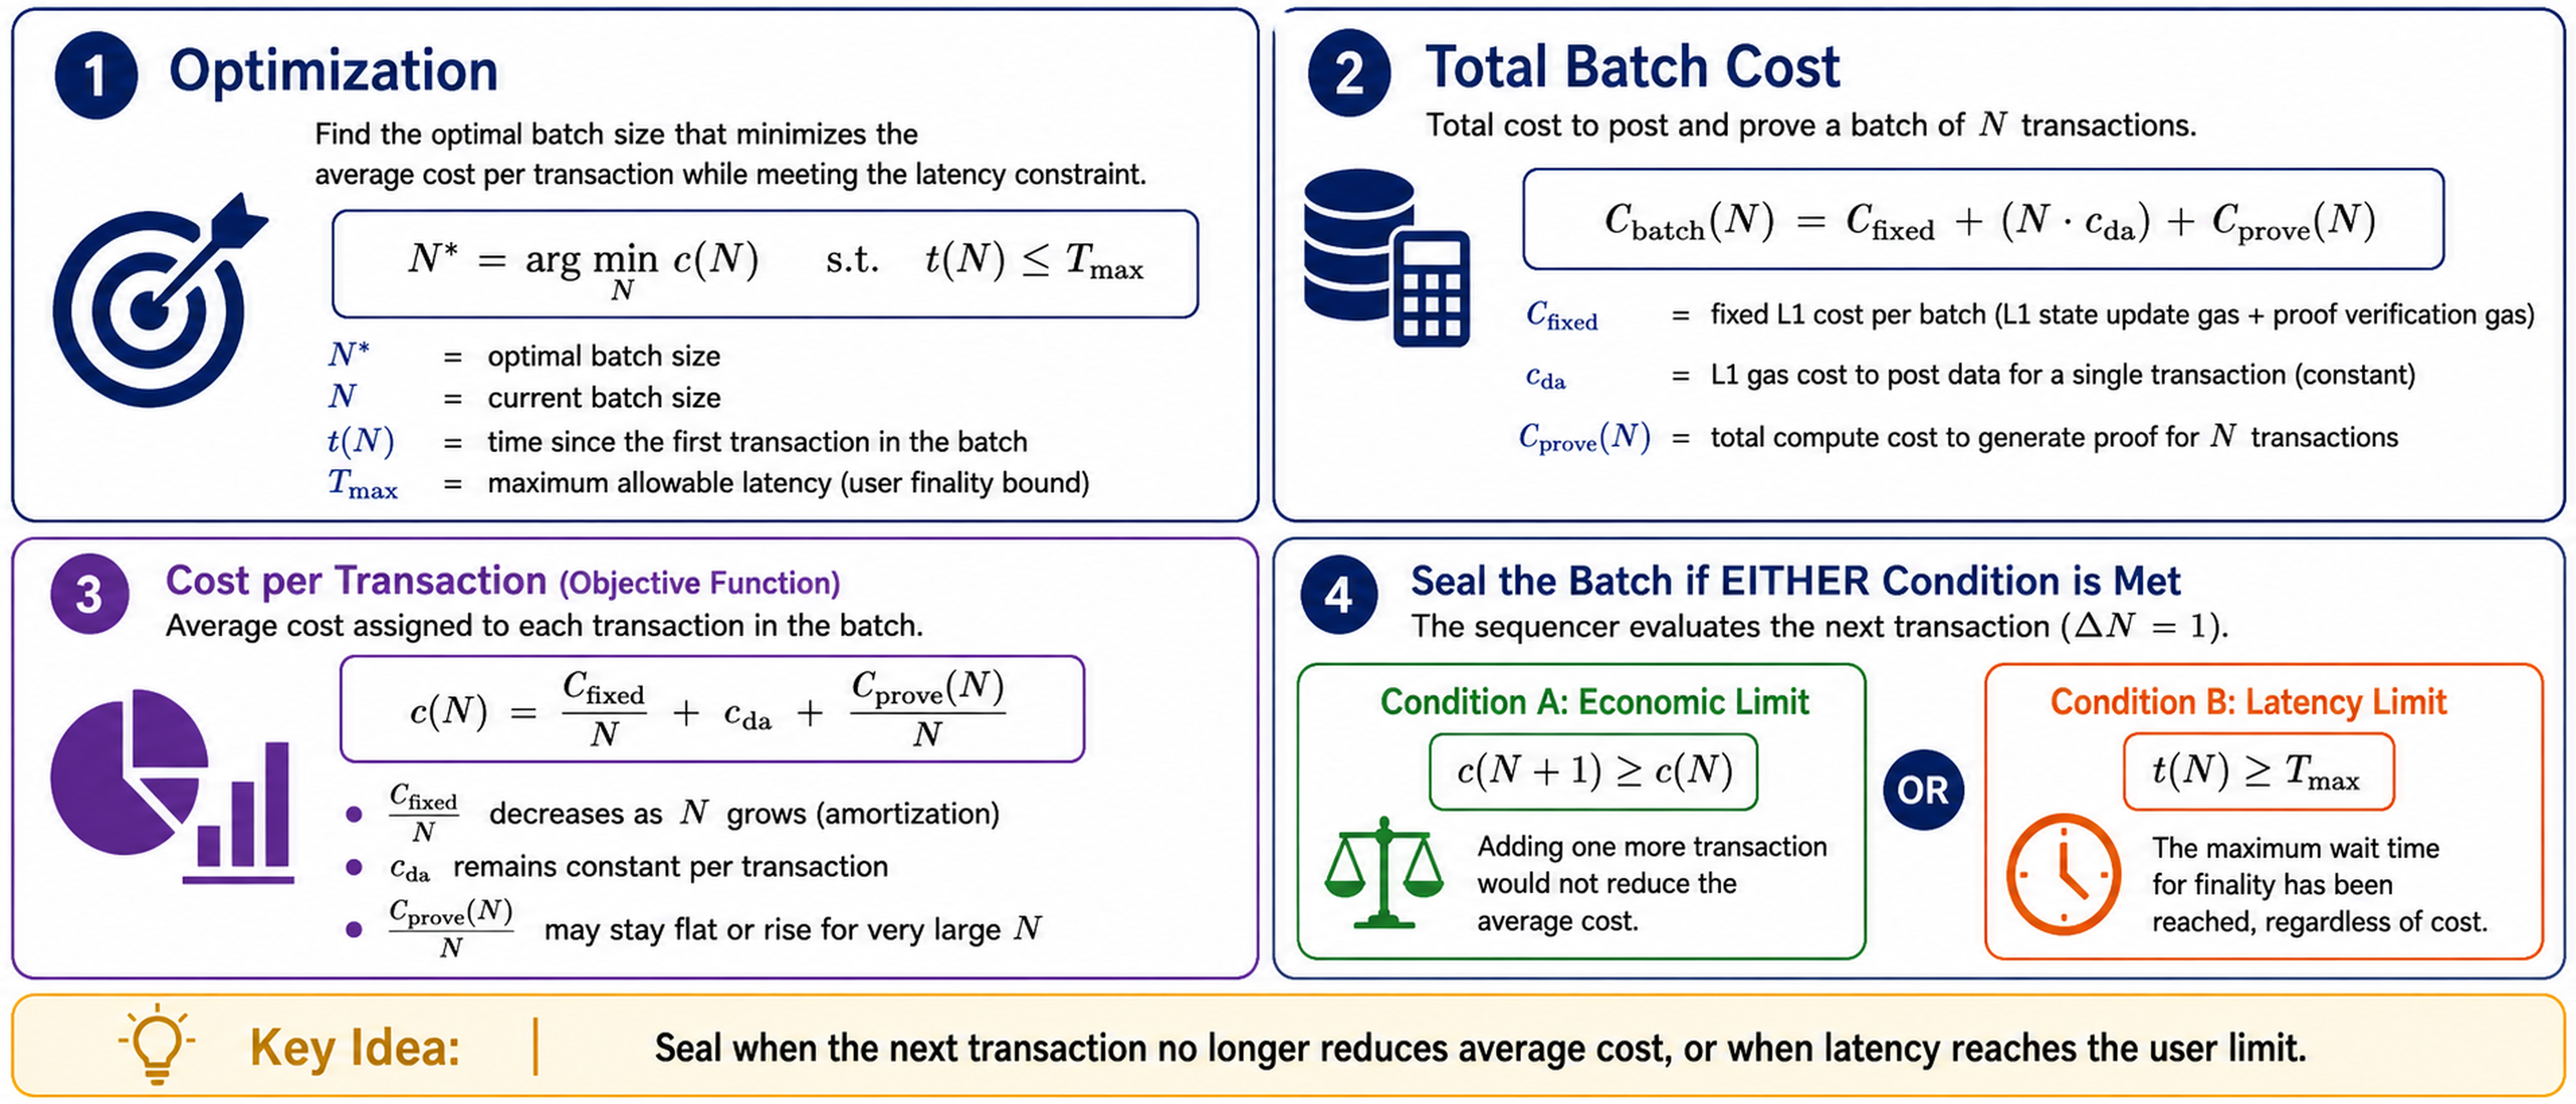
\includegraphics[width=1.1\linewidth]{poster/images/upscaled/dynamic_4x.png}
\begin{itemize}[leftmargin=0.75em,itemsep=0.08em,topsep=0pt,parsep=0pt]

\end{itemize}
\vspace{-2.6em}


% \[
% N^*=\arg\min_{N_{\min}\leq N\leq N_{\max}} U(N)
% \]

% \vspace{-0.6em}

% \[
% U(N)=Cost(N)+\gamma \cdot Latency(N)
% \]

% \vspace{-0.6em}

% \[
% Cost(N)=\frac{C_{\mathrm{fixed}}+\mathrm{BlobCost}(N)}{N}
% \]

% \vspace{-0.6em}

% \[
% Latency(N)=\frac{N}{2\lambda}+P(N)+T_{L1}
% \]

% \vspace{-0.5em}

% \begin{itemize}[leftmargin=0.8em,itemsep=0.1em,topsep=0pt]
%     \item Balances L1 cost, blob DA cost, waiting time, and proof delay.
%     \item Captures blob step-costs when batches cross blob-size limits.
%     \item Analytical model for benchmarking, not a production optimizer.
% \end{itemize} 
}

